\documentclass[titlepage=firstiscover, bibliography=totoc, captions=tableheading, parskip=half]{scrbook}
\titlehead{
  \centering
  
\includegraphics[scale=2.3]{pics/logo.png}
}
\author{Felix Geyer \\
  \texorpdfstring{\href{mailto:felix.geyer@tu-dortmund.de}{felix.geyer@tu-dortmund.de}}{}
  }
\title{Projektbericht zum Seminar: Maschinelles Lernen}
\publishers{TU Dortmund - Fakultät Physik}
\date{Abgabe: 15. Februar 2019}
\usepackage[aux]{rerunfilecheck}
\usepackage{polyglossia}
\setmainlanguage{german}
\usepackage{amsmath}
\usepackage{amssymb}
\usepackage{mathtools}
\usepackage{fontspec}
\usepackage[version=4]{mhchem}
\usepackage{scrhack}
\usepackage{float}
\floatplacement{table}{htbp}
\floatplacement{figure}{htbp}

\usepackage[locale=DE, separate-uncertainty=true, per-mode=reciprocal, decimalsymbol=comma]{siunitx}
%\usepackage{siunitx}
\DeclareSIUnit\px{px}

\usepackage[sorting=none]{biblatex}
\addbibresource{content/lit.bib}

\usepackage[section, below]{placeins}
\usepackage[labelfont=bf,
font=small,
width=0.9\textwidth,
format=plain,
indention=1em]{caption}
\usepackage{graphicx}
\usepackage{grffile}
\usepackage{subcaption}

\usepackage[math-style=ISO, bold-style=ISO, sans-style=italic, nabla=upright, partial=upright]{unicode-math}
\setmathfont{Latin Modern Math}

\usepackage[autostyle]{csquotes}

\usepackage[unicode]{hyperref}

\usepackage{mathtools}
\DeclarePairedDelimiter\abs{\lvert}{\rvert}

\usepackage{bookmark}

\usepackage{booktabs}

\usepackage{rotating}

\usepackage{tikz}
\usetikzlibrary{positioning}

\newcommand\JPsi{$J/\Psi$}
\newcommand\zerfall{$\beta$-Zerfall }
\newcommand\zerfalls{$\beta$-Zerfalls}
\newcommand\SppS{$\symup{Sp\bar{p}S}$}
\newcommand\barparen[1]{\overset{(-)}{#1}}

\begin{document}

\maketitle
  \section{Input und Struktur des Neuronalen Netzes}

  \begin{frame}[noframenumbering]
    \tableofcontents[currentsection]
  \end{frame}

  \begin{frame}{Struktur des Neuronalen Netzes (MiniDogNN)}
    \begin{figure}
      \centering
      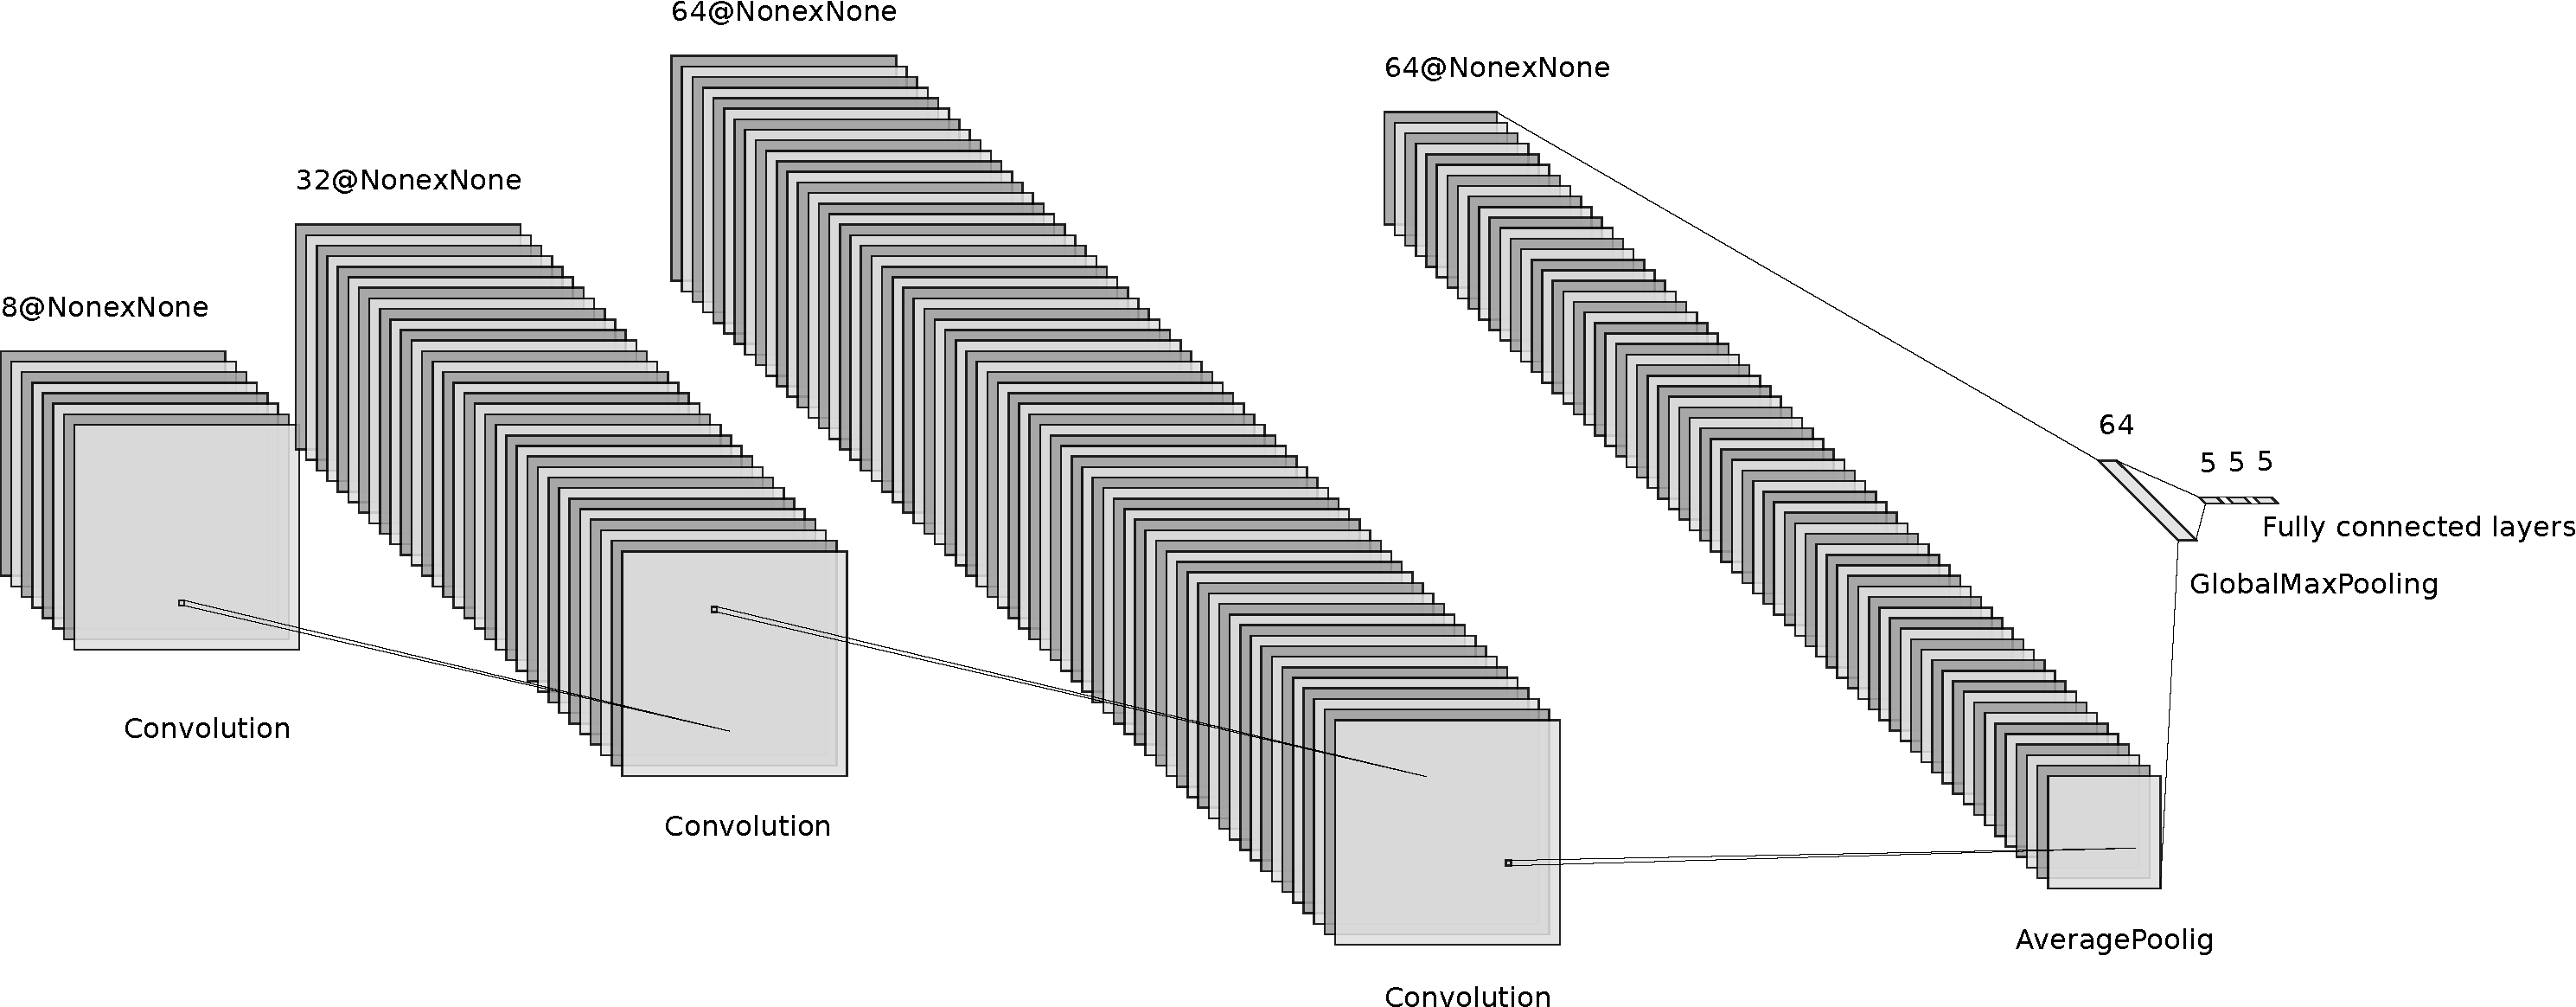
\includegraphics[width=0.9\textwidth]{logos/nn.pdf}
      %\caption{Plot.}
      \label{fig:1}
    \end{figure}
  \end{frame}
  \begin{frame}{Input des NN}
    \begin{figure}
      \centering
      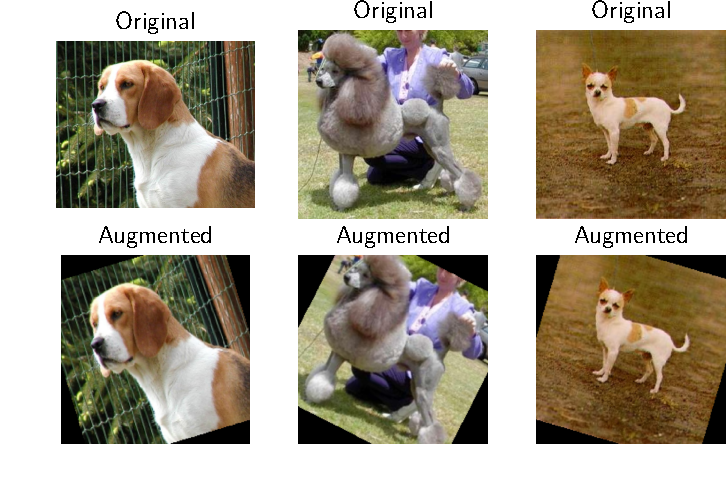
\includegraphics[width=0.7\textwidth]{logos/subplot.pdf}
      %\caption{Bilder vor und nach der Data Augmentation.}
      \label{fig:input}
    \end{figure}
  \end{frame}

  \section{Loss- und Accuracy-Kurven}

  \begin{frame}[noframenumbering]
    \tableofcontents[currentsection]
  \end{frame}

  \begin{frame}{MiniDogNN}
    \begin{columns}[c]
      \column{0.5\textwidth}
      \begin{figure}
        \centering
        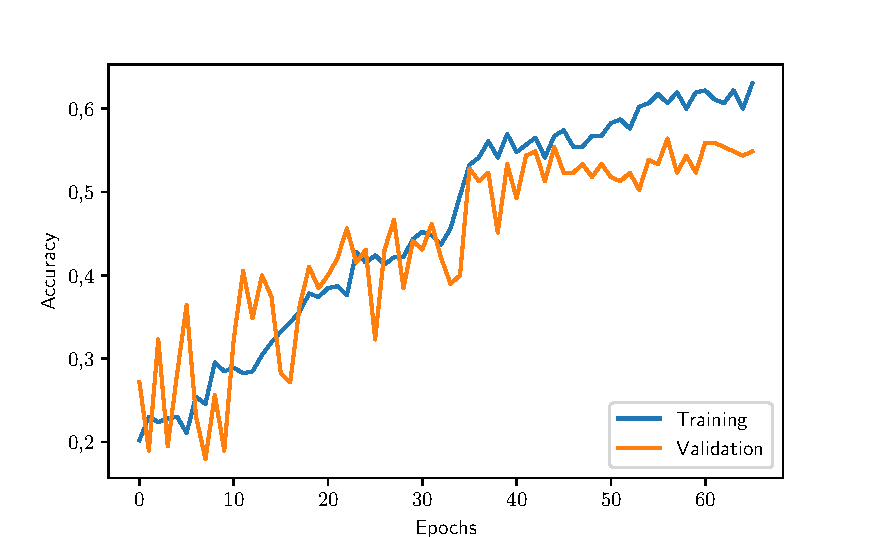
\includegraphics[width=\textwidth]{logos/MiniDogNN/history_acc_mini.pdf}
        % \caption{}
        \label{fig:acc_mini}
      \end{figure}
      \column{0.5\textwidth}
      \begin{figure}
        \centering
        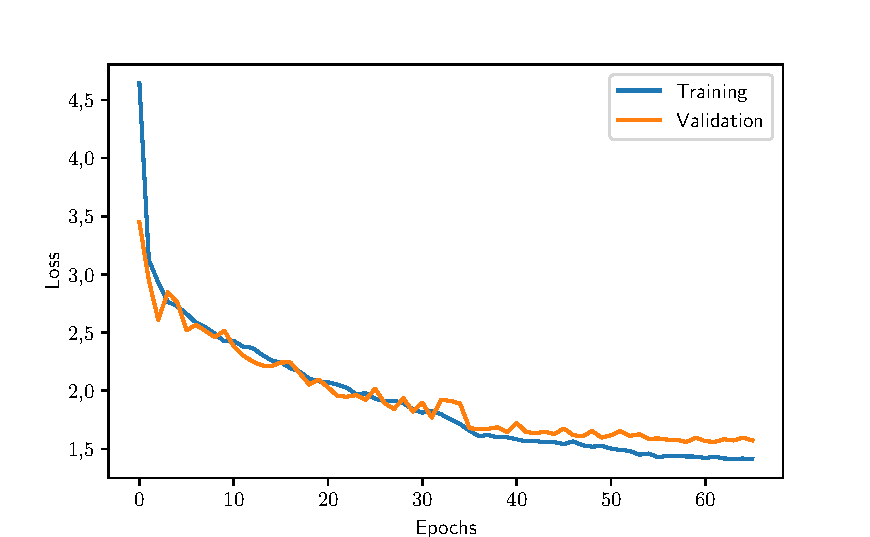
\includegraphics[width=\textwidth]{logos/MiniDogNN/history_loss_mini.pdf}
        % \caption{}
        \label{fig:loss_mini}
      \end{figure}
    \end{columns}
  \end{frame}

  \begin{frame}{PreDogNN}
    \begin{columns}[c]
      \column{0.5\textwidth}
      \begin{figure}
        \centering
        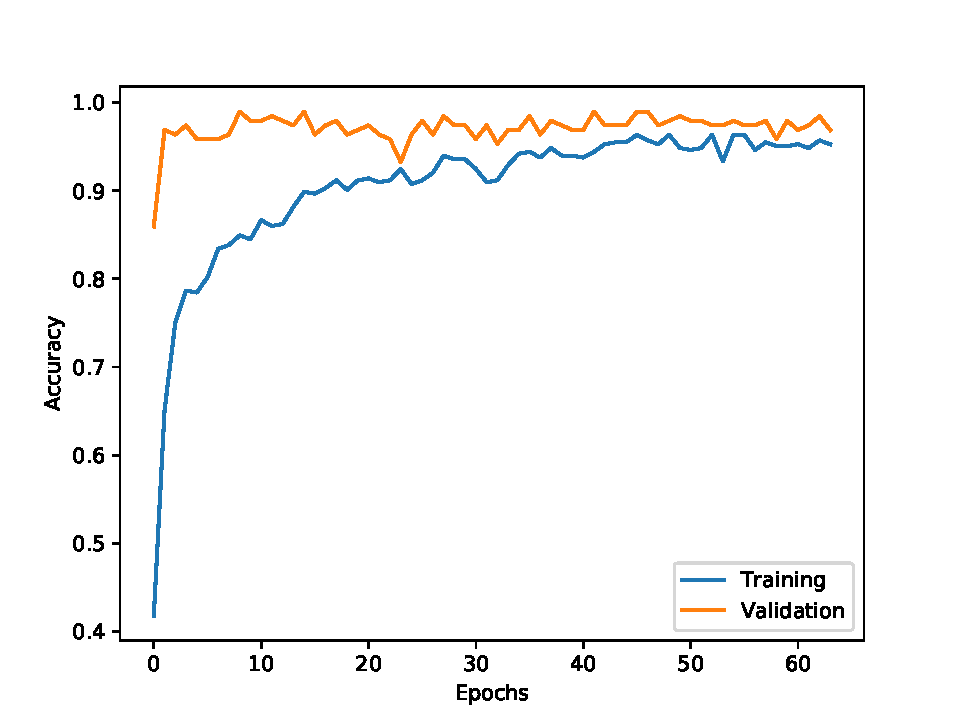
\includegraphics[width=\textwidth]{logos/PreDogNN/history_acc_pre.pdf}
        % \caption{}
        \label{fig:acc_pre}
      \end{figure}
      \column{0.5\textwidth}
      \begin{figure}
        \centering
        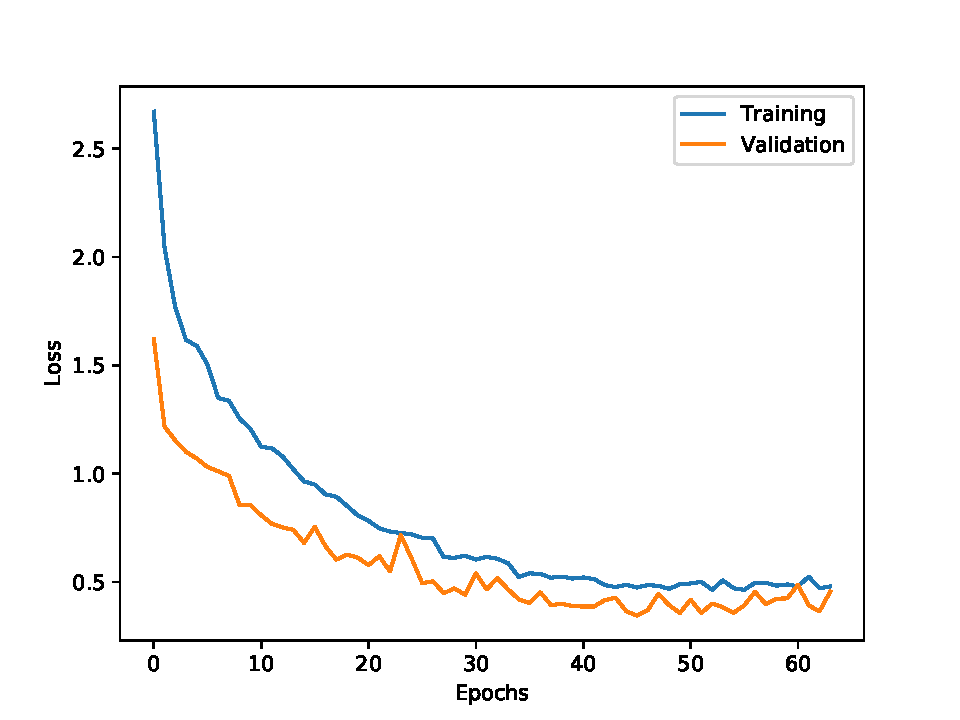
\includegraphics[width=\textwidth]{logos/PreDogNN/history_loss_pre.pdf}
        % \caption{}
        \label{fig:loss_pre}
      \end{figure}
    \end{columns}
  \end{frame}

  \begin{frame}{PreBigDogNN}
    \begin{columns}[c]
      \column{0.5\textwidth}
      \begin{figure}
        \centering
        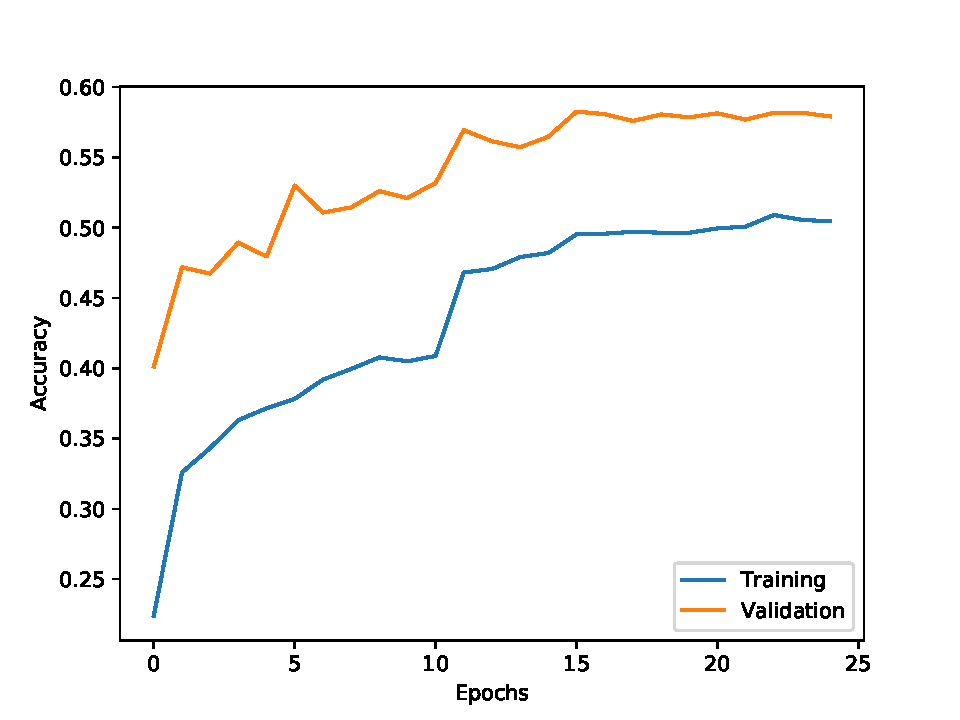
\includegraphics[width=\textwidth]{logos/PreBigDogNN/history_acc_prebig.pdf}
        % \caption{}
        \label{fig:acc_prebig}
      \end{figure}
      \column{0.5\textwidth}
      \begin{figure}
        \centering
        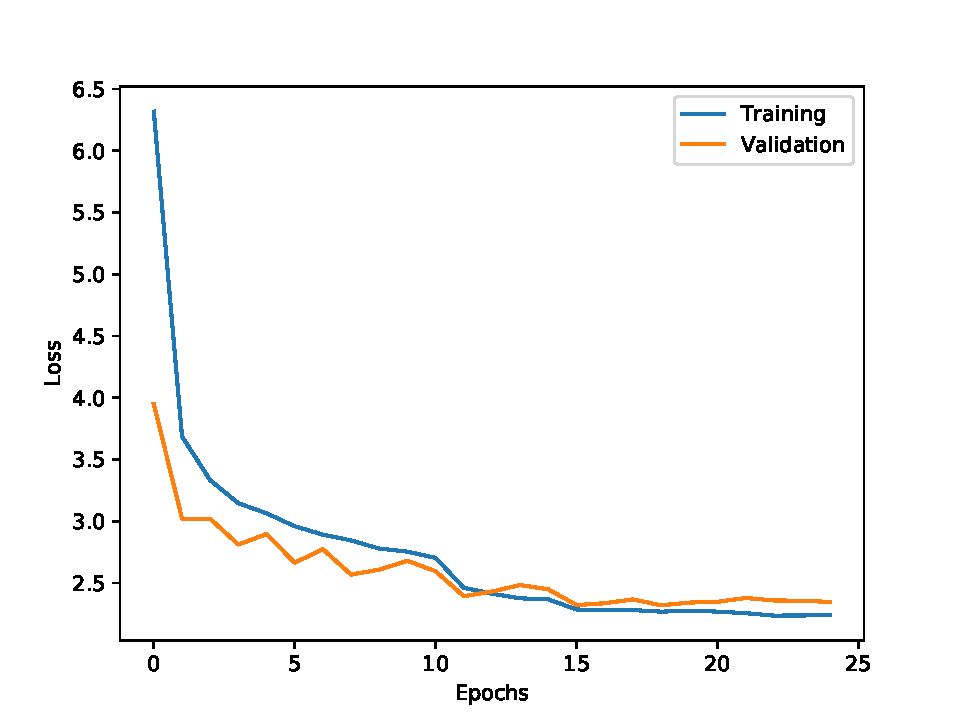
\includegraphics[width=\textwidth]{logos/PreBigDogNN/history_loss_prebig.pdf}
        % \caption{}
        \label{fig:loss_prebig}
      \end{figure}
    \end{columns}
  \end{frame}

  \section{Confusion Matrices}

  \begin{frame}[noframenumbering]
    \tableofcontents[currentsection]
  \end{frame}

  \begin{frame}{MiniDogNN ($n = 5$)}
    \begin{figure}
      \centering
      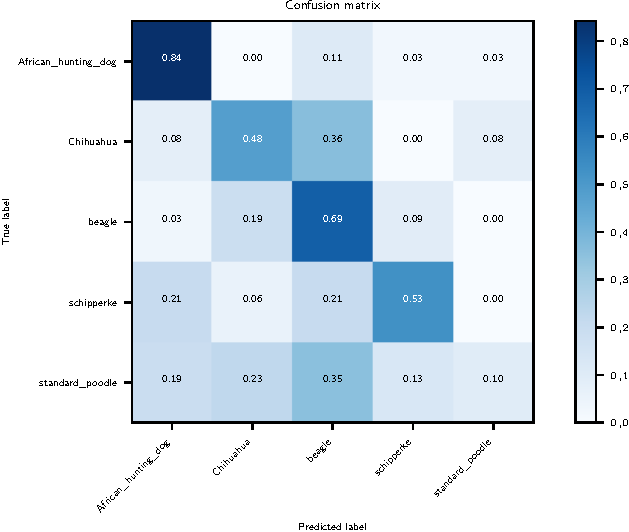
\includegraphics[width=0.5\textwidth]{logos/MiniDogNN/confusion_matrix_mini.pdf}
      % \caption{}
      \label{fig:cm_mini}
    \end{figure}
  \end{frame}

  \begin{frame}{MiniDogNN ($n = 120$)}
    \begin{figure}
      \centering
      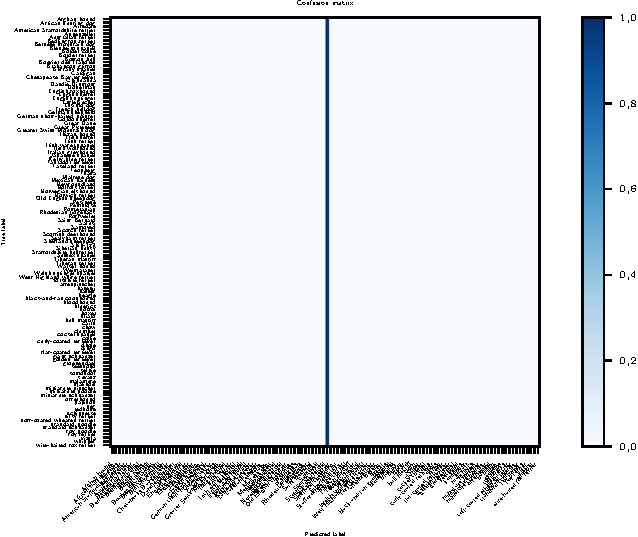
\includegraphics[width=0.5\textwidth]{logos/MiniDogNN/confusion_matrix_mini120.pdf}
      % \caption{}
      \label{fig:cm_mini120}
    \end{figure}
  \end{frame}

  \begin{frame}{PreDogNN}
    \begin{figure}
      \centering
      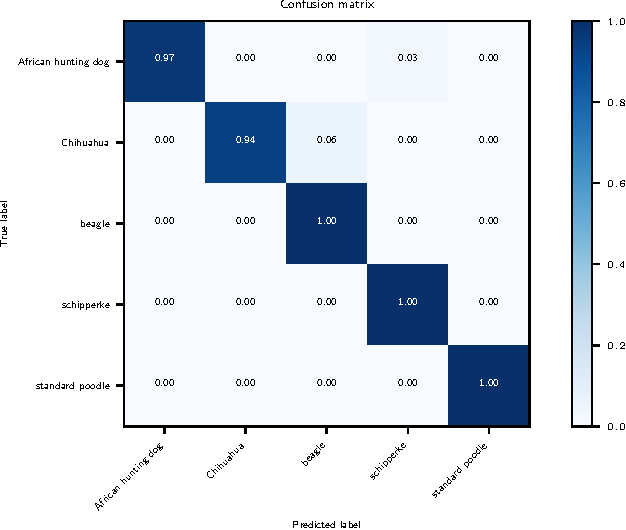
\includegraphics[width=0.5\textwidth]{logos/PreDogNN/confusion_matrix_PreDogNN.pdf}
      % \caption{}
      \label{fig:cm_pre}
    \end{figure}
  \end{frame}

  \begin{frame}{PreBigDogNN}
    \begin{figure}
      \centering
      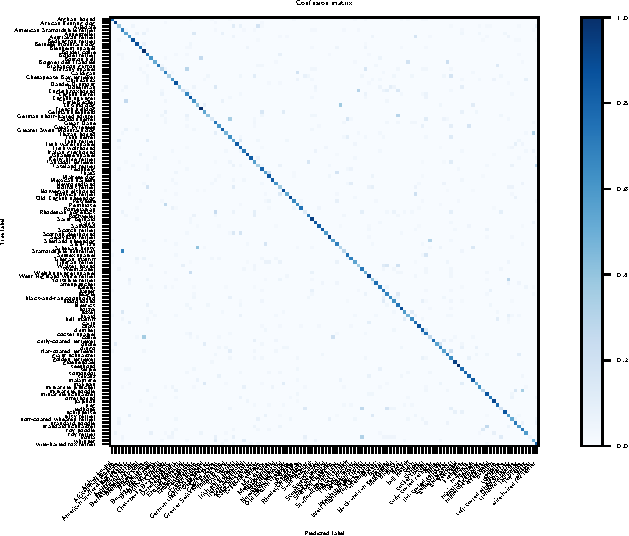
\includegraphics[width=0.5\textwidth]{logos/PreBigDogNN/confusion_matrix_bigpretrained.pdf}
      % \caption{}
      \label{fig:cm_prebig}
    \end{figure}
  \end{frame}

  \section{Alternativ-Methode Random Forest}

  \begin{frame}[noframenumbering]
    \tableofcontents[currentsection]
  \end{frame}

  \begin{frame}{Loss und Accuracy des Autoencoders ($n = 5$)}
    \begin{columns}[c]
      \column{0.5\textwidth}
      \begin{figure}
        \centering
        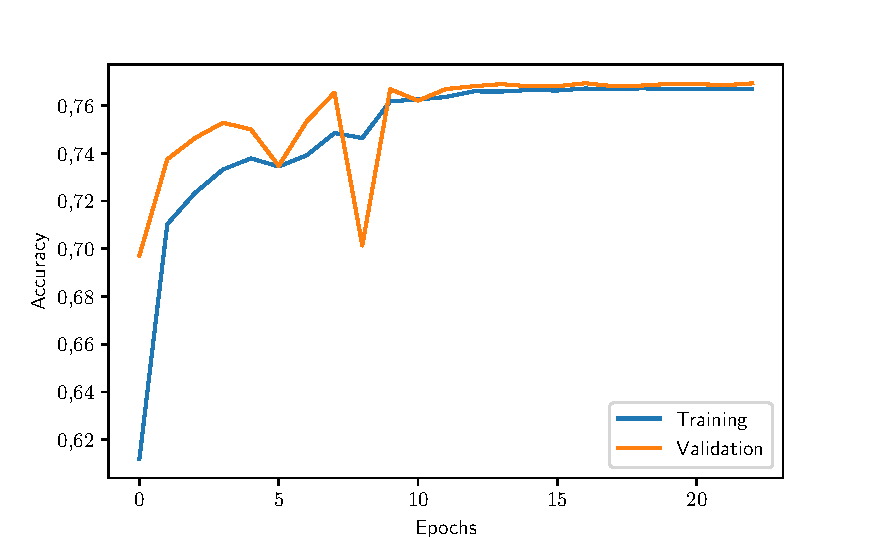
\includegraphics[width=\textwidth]{logos/RF/history_acc_rf.pdf}
        % \caption{}
        \label{fig:acc_rf}
      \end{figure}
      \column{0.5\textwidth}
      \begin{figure}
        \centering
        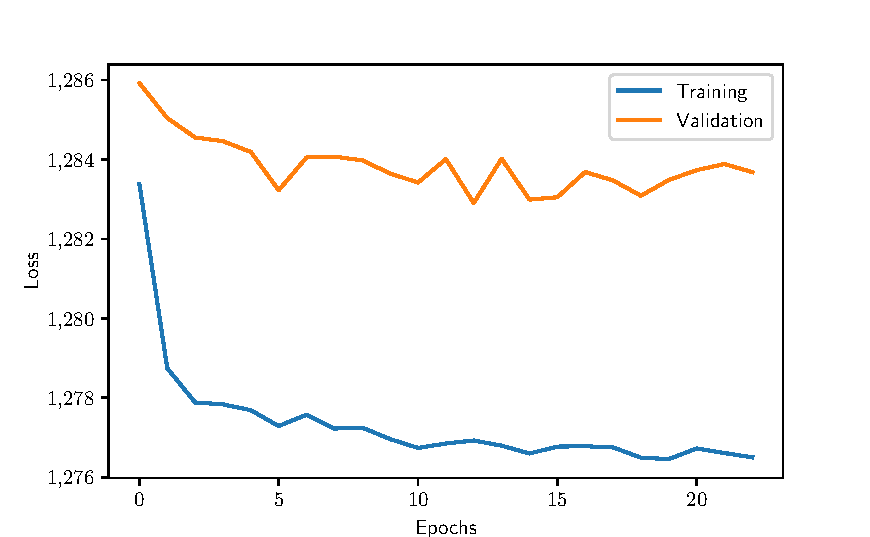
\includegraphics[width=\textwidth]{logos/RF/history_loss_rf.pdf}
        % \caption{}
        \label{fig:loss_rf}
      \end{figure}
    \end{columns}
  \end{frame}

  \begin{frame}{Confusion-Matrix ($n = 5$)}
    \begin{figure}
      \centering
      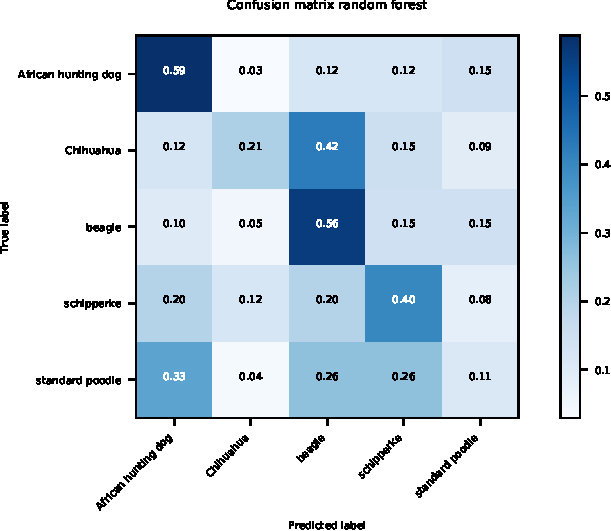
\includegraphics[width=0.5\textwidth]{logos/RF/confusion_matrix_rf.pdf}
      % \caption{}
      \label{fig:cm_rf}
    \end{figure}
  \end{frame}

\end{document}
